A Kalkulátor részben számítódik ki egy-egy interpolációnak az eredménye.
A megkapott adatok alapján számol, ha kell létre hozza a kezdő mátrixot, kiszámolja az eredmény mátrixot, majd annak segítségével kiszámolja a polinomot. \newline

\subsection{Felépítés}
	A számítást végző rész, nem áll sok fájlból, ezért ez nem lett sok részre szétbontva. 
	\begin{description}
		\item[calculator.cpp] 
		\hfill \\ Az egész számítás itt van megvalósítva, minden függvény, és segédfüggvény is.
		\item[erlang.cpp] 
		\hfill \\ Az Erlang-gal való kommunikáció megvalósítása
		\item[main.cpp] 
		\hfill \\ C++-os modul különálló tesztelésére kellett.
		\item[logTest.cpp] 
		\hfill \\ 
		Teszt függvények, melyekben dinamikus tesztesetek és paraméterezhető tesztesetek is vannak.
	\end{description}
\subsection{Fontosabb számítási függvények}
	%%\ref{fig:call_graph_caluclator_lagrange}
	\begin{figure}[h]
		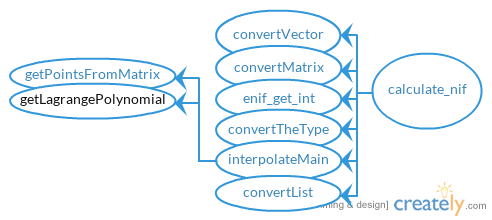
\includegraphics[width=10cm]{pics/call_graph_caluclator_lagrange}
		\centering
		\caption{Lagrange számítás hívási folyamata\label{fig:call_graph_caluclator_lagrange}}
	\end{figure}

	%%\ref{fig:call_graph_caluclator_newton}
	\begin{figure}[h]
		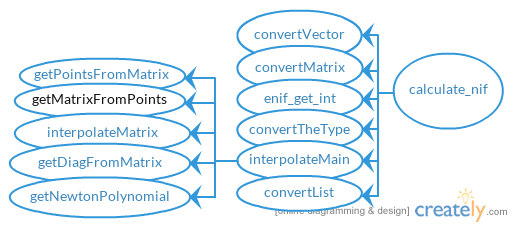
\includegraphics[width=10cm]{pics/call_graph_caluclator_newton}
		\centering
		\caption{Newton számítás hívási folyamata\label{fig:call_graph_caluclator_newton}}
	\end{figure}

	%%\ref{fig:call_graph_caluclator_hermite}
	\begin{figure}[h]
		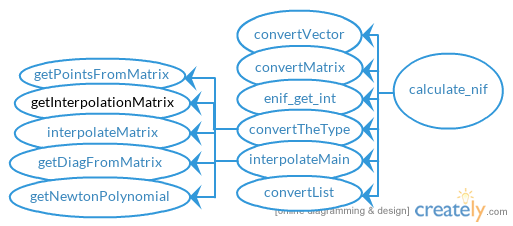
\includegraphics[width=10cm]{pics/call_graph_caluclator_hermite}
		\centering
		\caption{Hermite számítás hívási folyamata\label{fig:call_graph_caluclator_hermite}}
	\end{figure}

	\begin{description}
		\item[DArray interpolateMain] 
			\hfill \\ Kívülről meghívandó fő függvény mely elosztja és konvertálja a részeket
			\begin{description}
			  \item[DArray \&x :] Az x pontok listája 
			  \item[DMatrix \&Y :] Az x pontokhoz tartozó y pontok halmaza
			  \item[string type :] 
			  	Interpoláció típusa: Lagrange, Newton, Hermite
			  \item[bool inverse :] Inverz interpoláció kell-e
			\end{description}
		\item[void interpolateMatrix(DArray \&x, 	DMatrix \&M)] \hfill \\ 
			Interpolációs Táblázat kiszámítása
		\item[DArray l(int j, DArray X))] \hfill \\ 
			Lagrange polinom számítás segédfüggvénye
		\item[DArray getLagrangePolinomyal(DArray X, DArray Y)] \hfill \\ 
			Lagrange polinom számítás
		\item[DArray omega(int j, DArray X)] \hfill \\ 
			Newton polinom számítás segédfüggvénye
		\item[DArray polynomialAddition(DArray P, DArray Q)] \hfill \\ 
			polinom összeadás
		\item[DArray polynomialMultiply(DArray P, DArray Q)] \hfill \\ 
			polinom szorzás
		\item[DArray getPointsFromMatrix(DMatrix Y)] \hfill \\ 
			Pontokat(0. derivált) visszaadja a mátrixból
		\item[DMatrix getMatrixFromPoints(DArray Y)] \hfill \\ 
			Mátrixot ad vissza a pontokból
		\item[DArray getDiagFromMatrix (DMatrix \&M)] 
		\hfill \\
			Diagonális lekérése a mátrixból
		\item[void getInterpolationMatrix]
		\hfill \\  \textbf{(DArray X, DMatrix Y, DArray \&resX, DMatrix \&resM)}
		\hfill \\
			 X és Y ponthalmazból visszaadja a mátrixot 
	\end{description}
\subsection{Elosztott rendszerrel való kommunikáció}
	Az elosztott rendszerben hívódó számítást Erlang - erl\_nif"-el sikerült megoldanom. 
	Az ezzel kapcsolatos dolgokat az Calculator/erlang.cpp tartalmazza.
	\begin{description}
		\item[static ERL\_NIF\_TERM calculate\_nif] \hfill \\
		Ennek a függvénynek a segítségével valósul meg a kettő közötti kommunikáció
		\item[static int convertVector] \hfill \\
		Erlang lista C++ vektorrá konvertálása
		\item[static int convertMatrix] \hfill \\
		Erlang lista lista konvertálása C++ vektor vektorrá
		\item[static ERL\_NIF\_TERM convertList] \hfill \\
		Erlang listává konvertálás egy C++ vektorból
		\item[convertTheType] \hfill \\
			típus számot konvertálja string-gé: 
			"newton", "hermite", "lagrange"
		\item[static ErlNifFunc nif\_funcs] \hfill \\
			Felsorolja milyen függvényeket importálunk az Erlang-ba
	\end{description}
	Calculator/calculator.erl fájl tartalmazza az alábbi függvényeket: 
	\begin{description}
		\item[calculator:init()] \hfill \\
			"erlang:load\_nif" segítségével betölti a lefordított c++ fájlt.
		\item[calculator:calculate(\_X, \_Y, \_Type, \_Inverz)] \hfill \\
			Erre a függvényre lesz ráfordítva a C++-os függvény.
		\item[calculator:calculateByData(DataSetElement)] \hfill \\
		A bejövő paraméterből kinyeri a pontokat és a típust, majd meghívja a számító függvényt.
	\end{description}